\section{L'estimation d'un projet}

%*****************************************************************
\subsection{Pourquoi estimer ?}
\frame{\frametitle{Pourquoi estimer ?}

\vspace{.5cm}
\begin{itemize}
\item Cerner la durée du projet\\
\vspace{.2cm}
\item Déterminer les ressources à mettre en {\oe}uvre\\
\vspace{.2cm}
\item Déterminer la faisabilité technique du projet\\
\vspace{.2cm}
\item Pouvoir négocier\\
\vspace{.2cm}
\item \'{E}viter les dérives de coûts\\

\end{itemize}
\vfill
}
%*****************************************************************

\subsection{Estimer à différents niveaux} 
\frame{\frametitle{Estimations à différents niveaux}

\begin{itemize}

\item<+-> Niveau projet
 \begin{itemize}	
     \item	déterminer enveloppe budgétaire\\
     \item	poids du projet en termes d'effort\\
     \item	estimation de la rentabilité\\
     \item  évaluer une durée vraisemblable\\
 \end{itemize}

\item<+->Niveau étape
 \begin{itemize}	
	\item ajuster le découpage\\
	\item sous-traiter\\
	\item prévoir ressources\\
	\item prévoir délais pour planifier l'ordonnancement\\
 \end{itemize}

\item<+-> Niveau phase
 \begin{itemize}	
	\item planification précise\\
	\item calendrier des fournitures intermédiaires\\
	\item prévoir suivi de projet \\
	\item prévoir les montées/baisses en charge \\
\end{itemize}

\item<+-> Niveau tâche 
 \begin{itemize}	
	\item évaluer les tâches (souvent individuelles)  \\
 \end{itemize}
\end{itemize}
}

%*****************************************************************
\subsection{Règles empiriques de durée}
\frame{
\frametitle{Règles empiriques de durée}
\begin{columns}
%-- col left
\begin{column}{.55\textwidth}
\begin{itemize}
\item<+-> Tâche trop courte : se noyer dans les détails 
\item<+-> $\rightarrow$ minimum : 10 fois la granularité du projet.\\
\vspace{1cm}

\item<+-> Tâche trop longue : effet tunnel
\item<+-> $\rightarrow$ maximum : 3 fois la durée de la période d'avancement\\
\end{itemize}
\end{column}
%-- col right
\begin{column}{.45\textwidth}
	\onslide<3-4>{
		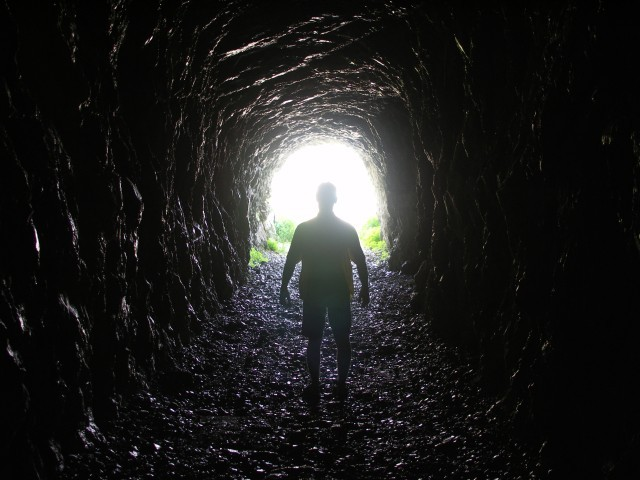
\includegraphics[width=.9\textwidth]{fig/tunnel.jpg}
	}
\end{column}
\end{columns}
}
%*****************************************************************
\subsection{Estimer charges et coûts}
\frame{\frametitle{Unité de charge}

\begin{itemize}
\item
La \emph{charge} est la quantité de travail exprimée en $ressources \times temps$.

\item Les  $ressource$ sont souvent des \textbf{hommes}\\

\item Le $temps$ est le
       \begin{itemize}
       \item[--] \textbf{mois} pour les grands projets, 
       \item[--] \textbf{jour} pour les petits projets.
       \end{itemize}

\item La charge est souvent pondérée par coefficient de productivité (e.g 1,20).
\end{itemize}
\vspace{.3cm}
Exemple : 10 jours $\times$ hommes \\ 
$\Leftrightarrow$ 1 homme pendant 10 jours\\ 
$\Leftrightarrow$ 10 hommes pendant 1 jour\\ 
$\Leftrightarrow$ 5 hommes pendant 2 jours\\
$\Leftrightarrow  \cdots$ \\
}
	
%***************************************************************** 
\subsection{Utiliser une méthode ?}
\frame{\frametitle{Utiliser une méthode ?}

\vspace{1cm}
\begin{itemize}
\item méthodes basées sur un \textbf{jugement d'expert}\\
      toujours applicable, n'importe quel domaine
\vspace{1cm}
\item méthodes de \textbf{répartition proportionnelle}\\
      applicable dans les domaines où des experts ont classifié la répartition
\vspace{1cm}
\item méthodes basées sur un \textbf{modèle de calcul}\\
      applicable quand un modèle quantitatif à été établi, indicateurs numériques nécessaires
\end{itemize}

\vfill
}
%*****************************************************************
\frame{
\frametitle{"Méthode" Delphi}

\begin{itemize}
\item Chaque expert donne anonymement une estimation
\item Les résultats sont rassemblés et exposés au groupe  
\item Chaque expert argumente sur son estimation
\item Les experts s'accordent sur une estimation consensuelle
\end{itemize}

}
%*****************************************************************
\frame{\frametitle{Méthode de répartition proportionnelle}

\vspace{-.5cm}
\[\begin{tabular}{|l|l|}
\hline
Etape		& Ratio		\\
\hline
Etude préalable	& 10\% du projet	\\
Etude détaillée	& 20 à 30\% du projet\\
Etude technique	& 5 à 15\% de la charge de réalisation \\
Réalisation	& 2 fois la charge d'étude détaillée\\
Mise en {\oe}uvre & 30 à 40\% de la charge de réalisation\\
\hline
\end{tabular}\]
\[\begin{tabular}{|l|l|}
\hline
Phase		&  Ratio		\\
\hline
Observation	& 30 à 40\% de l'étude préalable	\\
Conception/Organisation	& 50 à 60\% de l'étude préalable \\
Appréciation	& 10\%  de l'étude préalable \\
\hline
\end{tabular}\]
\[\begin{tabular}{|l|l|}
\hline
Tâche		&  Ratio		\\
\hline
Observation	& 30 à 40\%  	\\
Conception/Organisation	& 50 à 60\%  \\
Appréciation	& 10\%   \\
\hline
\end{tabular}\]

}
%*****************************************************************
\frame{\frametitle{Méthode modèle de calcul}
%\epsffile{estimation.ps}
\input estimation.pdftex_t

\vfill
}

%***************************************************************** 
\frame{\frametitle{Méthode COCOMO}
\vspace{1cm}
Soit $t$ le nombre de milliers de lignes de code livrées (sans les commentaires). Le type de projet est alors :

\[\begin{tabular}{|c|c|}
\hline
taille $t$ 	& type de projet	\\
\hline
$ t \leq 50$		&	simple	\\
$50 \leq t \leq 300$	&	moyen	\\
$ t > 300$		&	complexe\\
\hline
\end{tabular}\] 

La charge $c$ et le délai $d$ sont estimés par : 
\[\begin{tabular}{|l|cc|}
\hline
\hline
Type projet	& Charge en mois/homme & Délai en mois \\
\hline
simple		& $ c=3,2 \times t^{1,05}$ &	$d=2,5 \times c^{0,38}$ \\
moyen		& $ c=3 \times t^{1,12}$ &	$d=2,5 \times c^{0,35}$ \\ 
complexe	& $ c=2,8 \times t^{1,2}$ &	$d=2,5 \times c^{0,32}$\\
\hline
\hline	
\end{tabular}\]
\vfill
}
%***************************************************************** 
\frame{
\frametitle{Facteurs correcteurs COCOMO}

\begin{small}
\begin{tabular}{|l|l||c|c|c|}
\hline
		& Facteur		& bas & moy. & élevé\\
\hline
		& fiabilité requise	& 0,88	& 1	& 1,15	\\
Produit		& taille base données	& 0,95	& 1	& 1,08	\\
		& complexité produit	& 0,85	& 1	& 1,15	\\
\hline
		& contrainte temps d'exec. & - & 1	& 1,11 \\
Ordinateur	& contrainte taille mémoire & - & 1	& 1,06\\
		& instabilité logiciel de base	& 0,87 & 1 & 1,15\\

\hline
		& Expérience du domaine		& 1,13	& 1 & 0,91 \\
Personnel	& Qualification programmeur	& 1,17	& 1 & 0,86\\
		& Familiarité logiciel de base & 1,10 & 1 & 0,90\\
		& Expérience du langage		& 1,02	& 1 & 0,95\\
		
\hline
		& Utilis. méthode moderne	& 1,10	& 1	& 0,91\\
Projet		& Utilisation d'outils 		&	&	& \\
		& d'aide à la programmation & 1,10& 1	& 0,91\\
		& Contrainte de délais		& 1,08	& 1	& 1,04\\
\hline
\end{tabular}
\end{small}
\vfill
}
%*****************************************************************
\frame{\frametitle{Méthodes des points fonctionnels}

\begin{itemize}
\item Méthode proposée par A. Albrecht (IBM), norme AFNOR (XP Z 67-160), 
largement disséminée \url{http://www.ifpug.org/}.
 
\item L'estimation de la complexité du système à developper, l'est à partir des \emph{fonctions} du futur système.

\item Chaque fonction 
\begin{itemize}
\item fait partie d'une des 5 unités d'{\oe}uvres définies (relatives aux entrées/sorties ou aux traitements) 
\item a un niveau de complexité (faible/moyen/élevé)
\end{itemize}
 
\item
\'{E}valuation en trois étapes :
\begin{enumerate}
\item calcul de la taille  
\item ajustement de la taille  
\item transformation du nombre de points de fonction en charge
\end{enumerate}


\end{itemize}
}
\begin{comment}
%*****************************************************************
\frame{\frametitle{Estimation des risques}
\vspace{1cm}

\underline{En général} : 
\begin{center}
Risque = Coût $\times$ Probabilité
\end{center}


\underline{Pour les S.I.} 
\begin{enumerate}
\item	taille du projet
\item 	difficulté technique
\item	degré d'intégration
\item	configuration organisationnelle
\item	le changement
\item	instabilité de l'équipe projet 
\end{enumerate}

\vfill
}
 
%*****************************************************************
\frame{\frametitle{Profil de risque}

\vspace{1cm}
\input risque.pdftex_t
\vfill
}
\end{comment}
%*****************************************************************	 
